\definecolor{bg}{rgb}{0.95,0.95,0.95}
\chapter{مقدمات و نکات امنیتی}
\section{مسائل مقدماتی در آزمایشگاه ریزپردازنده}

\subsection{قوانین آزمایشگاه ریزپردازنده}
به منظور افزایش کارایی درس آزمایشگاه ریزپردازنده، رعایت عدالت میان همه‌ی گروه های آزمایشگاه و آموزش حداکثری مطالب درس به صورت عمل، مدرسی و دانشجویان ملزم به رعایت نکات و قوانین زیر هستند:
\begin{enumerate}
    \item مدرسین و دانشجویان موظفند راس ساعت در کلاس حاضر شوند.
    \item غیبت در هیچ یک از جلسات آزمایشگاه مجاز نیست.
    \item آزمایش ها در گروه های دو نفره انجام می‌شوند.
    \item ارائه‌ی پیش گزارش به صورت انفرادی‌است و هر دانشجو موظف است برای هر آزمایش پیش‌گزارش آن را تهیه نماید. پیش‌گزارش شامل جواب سوال هایی که با رنگ قرمز در قسمت مقدمه‌ی هر آزمایش آمده می‌شود.
    \item نیازی به ارائه‌ی گزارش‌کار برای آزمایش ها نیست و تحویل خروجی صحیح به مدرس آزمایشگاه کفایت می‌کند.
\end{enumerate}

\subsection{آشنایی با بردبورد}

در دنیای سیستم های نهفته و مدار های الکترونیکی معمولا برای سریع تر شدن فرایند توسعه، ابتدا یک نمونه‌ی اولیه با بردبورد می‌سازند و بعد از توسعه‌ی محصول نهایی سراغ تهیه‌ی مدار چاپی و یا روش های دیگر می‌روند. ما نیز در آزمایشگاه ریزپردازنده آزمایش های گفته شده را با استفاده از بردبورد انجام می‌دهیم.
\begin{figure}[h]
    \centering
    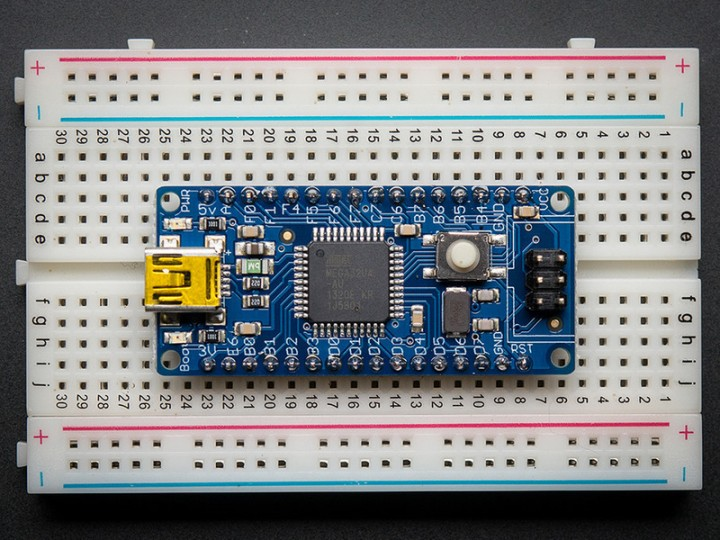
\includegraphics[width=6cm]{breadboard.png}
    \caption{تصویر یک بردبورد که روی آن یک میکروکنترلر قرار داده شده‌است.}
    \label{fig:breadboard}
\end{figure}

بردبورد در واقع یک مدار با اتصالات از پیش تعیین شده است، به طوری که سوراخ های میانی به صورت عمودی و سوراخ های دو ردیف بالا و پایین به صورت افقی به یکدیگر اتصال الکتریکی دارند. پیشنهاد می‌شود که از این دو ردیف برای اتصال مثبت و منفی منبع ولتاژ استفاده کنید. عمدتا در این درس مثبت و منفی از پین های \lr{5V} و \lr{GND} میکروکنترل تامین می‌شود اما می‌تواند به هر صورت دیگری نیز باشد. 

\subsection{آشنایی با بورد \lr{Arduino Uno}}

در این آزمایشگاه از بورد \lr{Arduino Uno} استفاده می‌کنیم. این بورد مبتنی بر میکروکنترلر \lr{ATmega328P} است که شامل ۱۴ پین خروجی و ورودی است که ۶ تا از آنها قابلیت خروجی \lr{PWM} و ۶ تا از آنها قابلیت خروجی آنالوگ دارند. همچنین این میکروکنترلر ۳۲ کیلوبایت حافظه‌ی فلش (که از آن ۰.۵ کیلوبایت برای برنامه‌ی بوتلودر استفاده شده) و ۲ کیلوبایت \lr{SRAM} و ۱ کیلوبایت حافظه‌ی \lr{EEPROM} دارد.
\lr{
\begin{center}
\begin{tabular}{ |c|c| } 
 \hline
 \lr{Microcontroller} & \lr{ATmega328P} \\ 
  \hline
 \lr{Operating Voltage} & \lr{5V} \\ 
  \hline
 \lr{Input Voltage (recommended)} & \lr{7-12V} \\ 
  \hline
 \lr{Input Voltage (limit)} & \lr{6-20V} \\ 
  \hline
 \lr{Digital I/O Pins} & \lr{14 (of which 6 provide PWM output)} \\ 
  \hline
 \lr{PWM Digital I/O Pins} & \lr{6} \\ 
  \hline
 \lr{Analog Input Pins} & \lr{6} \\ 
  \hline
 \lr{DC Current per I/O Pin} & \lr{20 mA} \\
  \hline
 \lr{DC Current for 3.3V Pin} & \lr{50mA} \\
  \hline
\lr{ Flash Memory} & \lr{32 KB (ATmega328P) of which 0.5 KB used by bootloader} \\ 
 \hline
 \lr{SRAM} & \lr{2 KB (ATmega328P)} \\ 
  \hline
 \lr{EEPROM} &  \lr{1 KB (ATmega328P)} \\
  \hline
 \lr{Clock Speed} &  \lr{16 MHz} \\ 
 \hline
\end{tabular}
\end{center}
}
\begin{figure}[h]
    \centering
    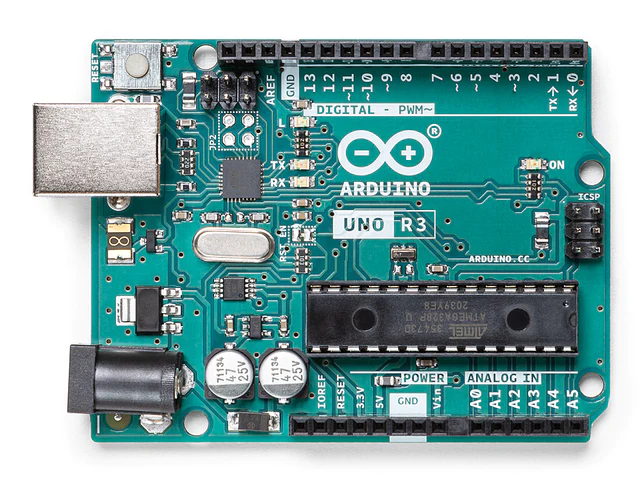
\includegraphics[width=8cm]{ArdUno.png}
    \caption{تصویری از بورد \lr{Arduino Uno}}
    \label{fig:arduno}
\end{figure}

\subsection{آشنایی با محیط \lr{Arduino IDE}}
بورد های آردوینو را می‌توان به راحتی با استفاده از برنامه‌ی \lr{Arduino IDE} برنامه ریزی کرد و نقطه قوت اصلی آن نسبت به پلتفرم های دیگر نیز همین سهولت در برنامه ریزی آنهاست. در ابتدا شما باید ابتدا این برنامه را از \href{https://www.arduino.cc/en/software}{این لینک} دریافت کرده و نصب کنید و سپس آن را اجرا کنید.
پس از اجرای برنامه با محیط زیر روبرو می‌شوید:

\begin{figure}[h]
    \centering
    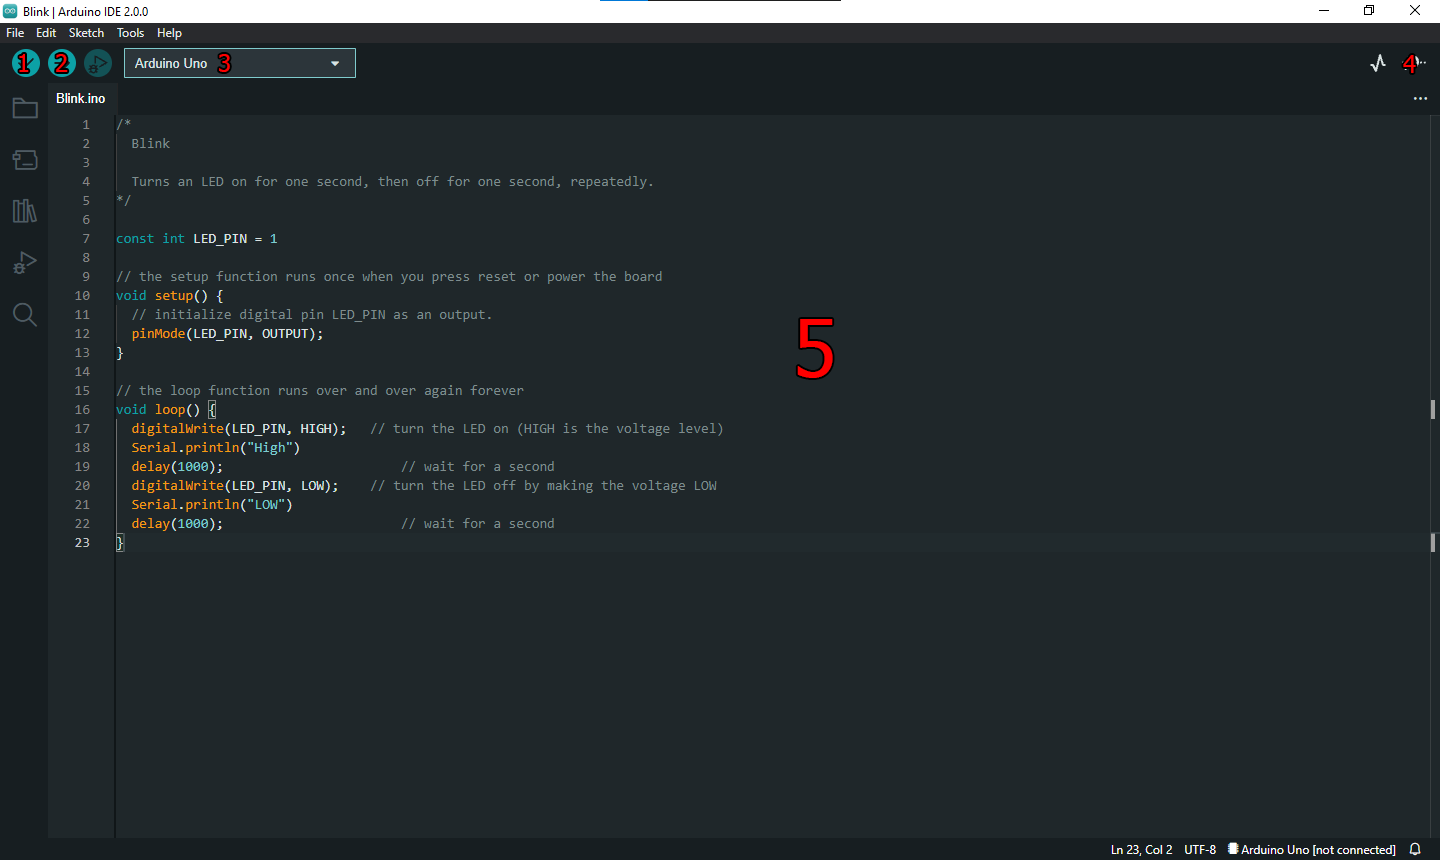
\includegraphics[width=16cm]{arduinoide1.png}
    \caption{تصویری از محیط \lr{Arduino IDE}}
    \label{fig:ardunoide}
\end{figure}

\begin{enumerate}
    \item کامپایل برنامه
    \item کامپایل برنامه و آپلود آن بر روی بورد
    \item انتخاب بورد
    \item سریال مانیتور
    \item ادیتور کد
\end{enumerate}

با این محیط در ویدیو های آموزشی که در اختیار شما قرار می‌گیرد بیشتر آشنا خواهیم شد.

\section{نکات امنیتی کار با قطعات الکترونیکی}

\subsection{دیود نوری}
دیود های نوری یک حداکثر جریان قابل تحمل دارند و اگر جریان عبور از آنها از یک مقدار معین بیشتر شود می‌سوزند. برای همین همواره از یک مقاومت سری حداقل ۱۰۰ اهمی برای محدود کردن جریان دیود استفاده می‌کنیم. در آزمایش اول بیشتر با نحوه‌ی محاسبه‌ی مقاومت مورد نیاز برای دیود های نوری آشنا می‌شویم.

\subsection{جریان خروجی از پین های میکروکنترلر}

پین های ورودی و خروجی میکروکنترلر ها محدودیت جریانی ۲۰ میلی‌آمپری دارند. توجه کنید و به هیچ وجه مداری نبندید که جریان خروجی از پین های میکروکنترلر از ۲۰ میلی‌آمپر بیشتر شوند. در غیر این صورت امکان خرابی قطعه وجود دارد و عواقب آن بر عهده‌ی خودتان است. برای اینکه مدار هایی با جریان عبوری بیشتر را توسط میکروکنترلر کنترل کنیم باید از ترانزیستور و یا رله استفاده کنیم که در آزمایش های آینده بیشتر با آن آشنا خواهیم شد.

\subsection{راهنمای پین های آردوینو}
\begin{figure}[h]
    \centering
    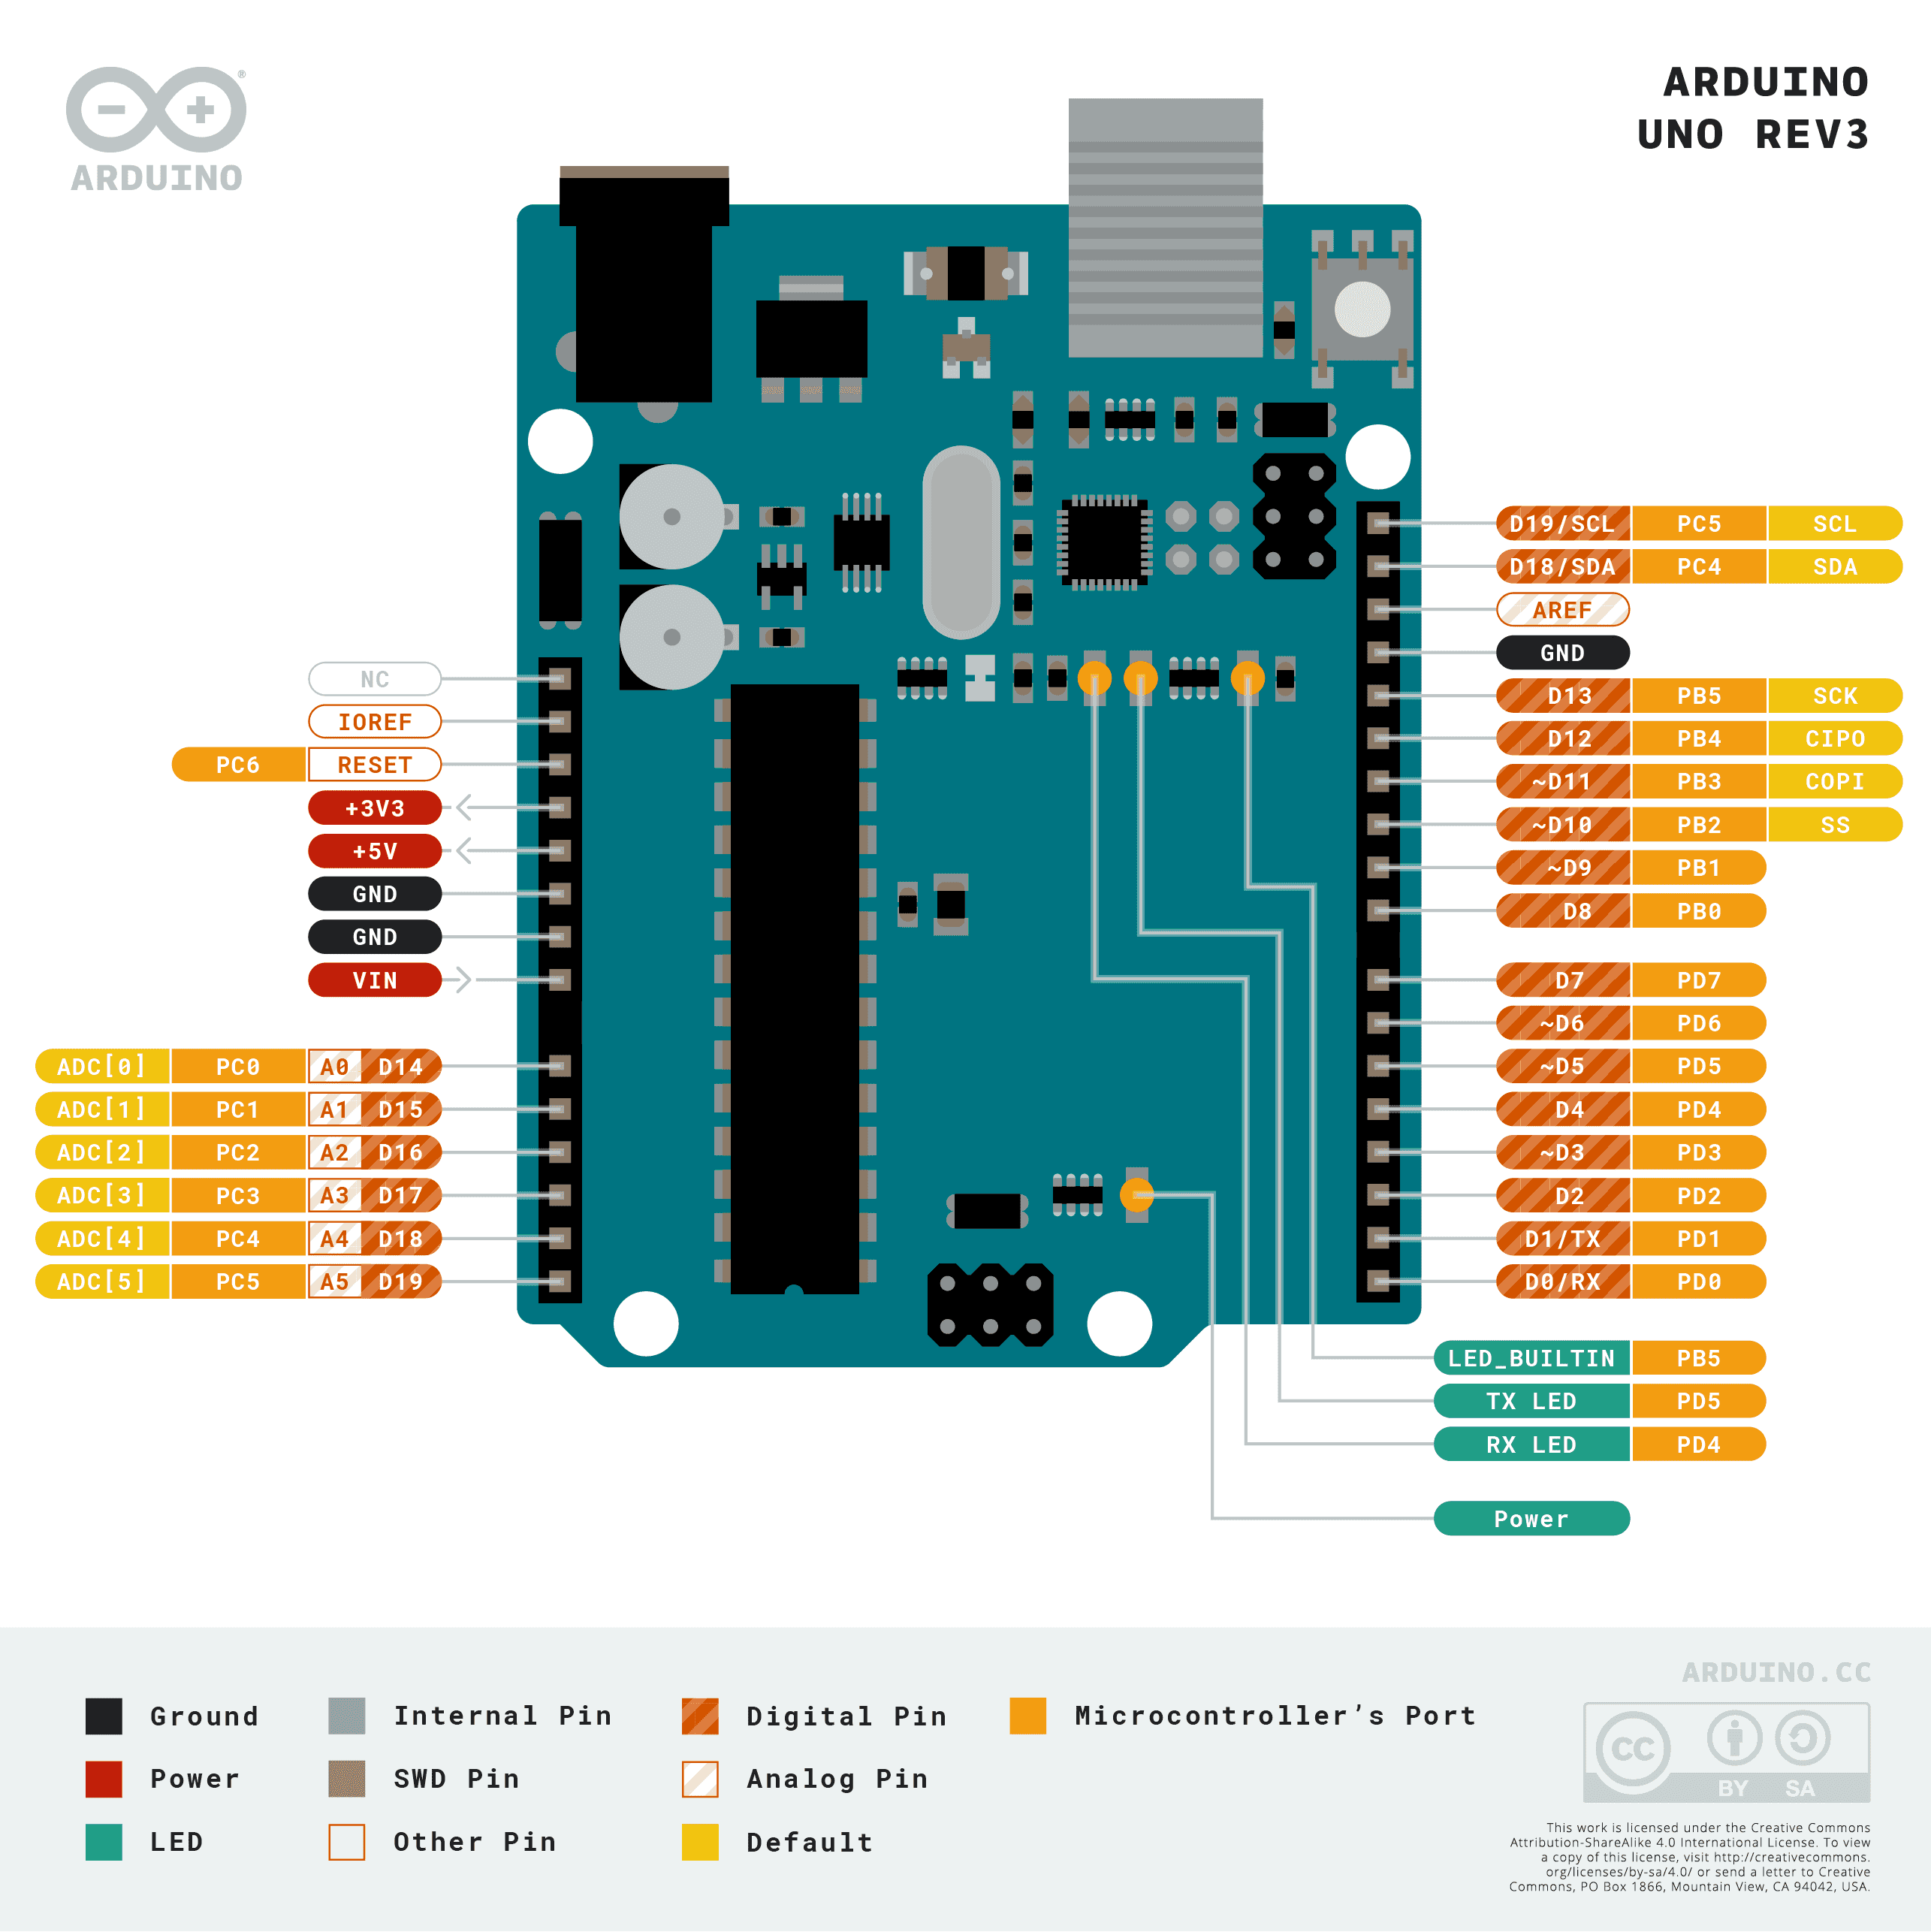
\includegraphics[width=16cm]{Pinout-UNO.png}
    \caption{راهنمای پین های آردوینو}
    \label{fig:ard_pinout}
\end{figure}

\